\chapter{Concept Learning}
In this chapter we will analyze our first learning algorithm, that is not used usually in pratice but it can be useful to discover 
some aspect behind and also we will briefly introduce the effect of bias in ML model.

We define \emph{Concept Learning} as 
\begin{defi}
    Concept Learning consist in infer a boolean-valued function from training examples of its input and output
\end{defi}
It can be also formulated as a problem of searching through a predefined space of potential hypothesis for the hypothesis that best fit 
the training examples and to better introduce we consider as an example the task to discover if our friend "Aldo" enjoys his favorite water sport,
with six features (Sky, AirTemp, Humidity, Wind, Water, Forecast), as we can note in figure \ref{img:conceptExample}, and also for each attribute
the hypothesis can be "?" (every value is acceptable), a single required value and "$\emptyset$" (no value is acceptable).

\begin{figure}
    \caption{Example of EnjoySport problem}
    \label{img:conceptExample}
    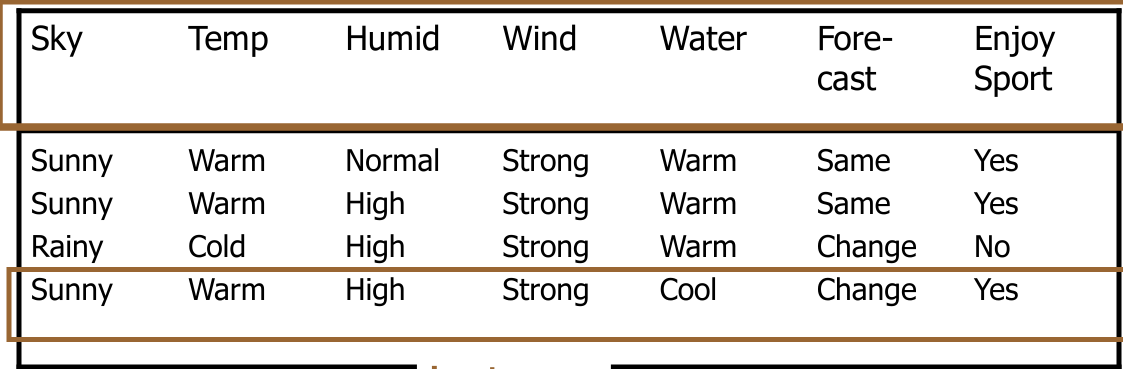
\includegraphics[width=\textwidth]{images/enjoySport}
\end{figure}
We define now an important concept, assumpted usually in all ML models, that is important to understand and remember
\begin{defi}[Inductive Hypothesis \cite{mitchell}]
    Any hypothesis found to approximate  the target function well over a sufficiently large set of training examples will also approximate the 
    target function well over other unobserved examples.
\end{defi}
Concept Learning can be viewed as the task of searching through a large space of hypotheses implicitly defined by the hypothesis representation and 
the goal of this search is to find the hypothesis that best fits the training examples.

We define our hypothesis $h: X \to \{0, 1\}$ that satisfi4es $x$ when $h(x) = 1$ and it is consistent with our training examples $D$ if $h(x) = y \, \forall (x, y) \in D$,
so the object of concept learning is to find an hypothesis that is consistent and fits better the training examples.

Many algorithms for concept learning use a general-to-specific ordering of hypothesis to achieve a fast training, so we have
\begin{defi}
	Let $h_j$ and $h_k$ be boolean-valued functions defined over $X$, then $h_j$ is more general than or equal to $h_k (h_j \geq _G h_k)$ if and only if 
	\[ \forall x \in X h_k(x) = 1 \to h_j(x) = 1 \]
\end{defi}
Note that $\geq _G$ relation is defined independent of the target concept, they depends only on which instances satisfy the two hypothesis, and also 
this defines a partial order over the hypothesis space $H$, useful in concept learning algorithms that we will introduced and analyzed in the following paragraph.

\section{Find-S}
The Find-S algorithm exploits the most general than or equal approach to efficiently conduct a search consistent $h$, without have to enumerate all $h$ in hypothesis space $H$,
and in figure \ref{alg:find-S} it is possible to note the pseudocode of Find-S Algorithm and in \ref{img:find-S} there is an example of execution of Find-S.

\begin{figure}
	\caption{Pseudocode of Find-S algorithm}
	\label{alg:find-S}
	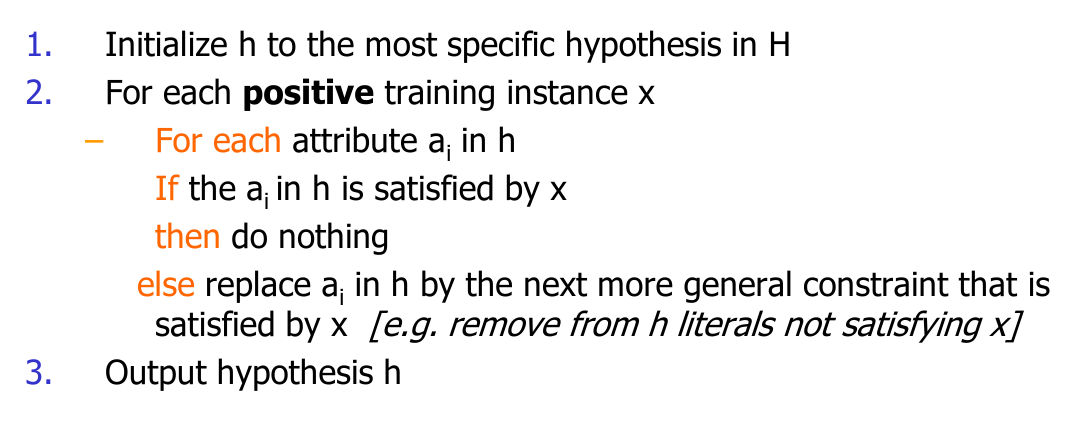
\includegraphics[width=\textwidth]{images/find-S-pseudo}
\end{figure}

\begin{figure}
	\caption{Example of Find-S execution}
	\label{img:find-S}
	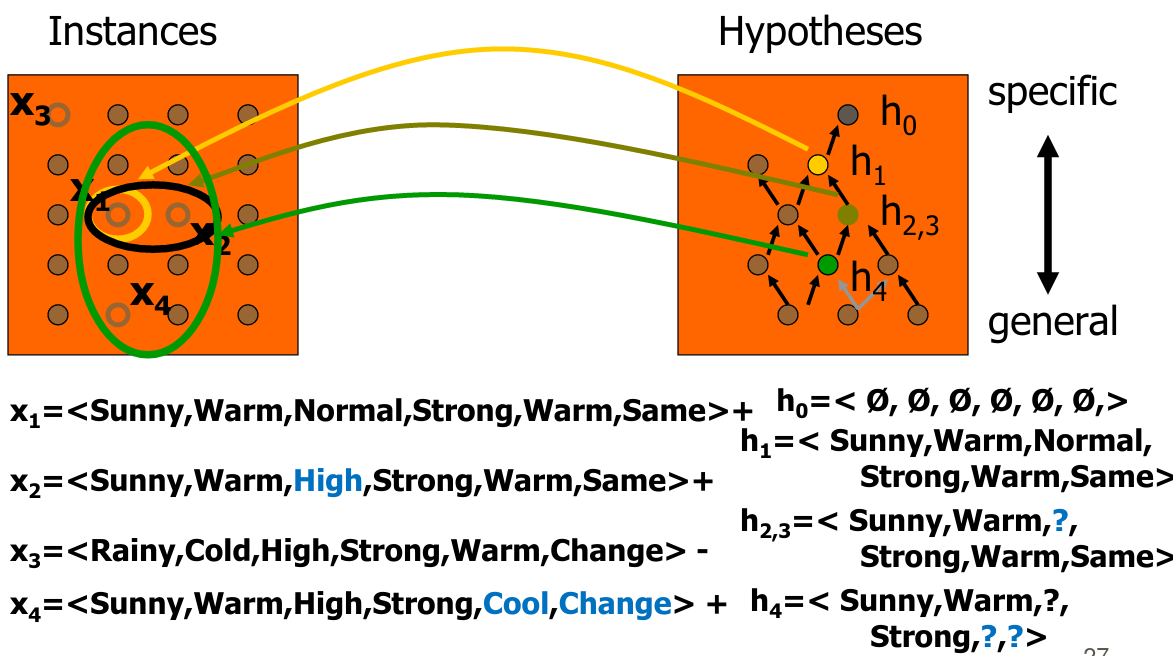
\includegraphics[width=\textwidth]{images/find-S-example}
\end{figure}
Hypothesis space is described by conjunctions of attributes and Find-S will output the most specific hypothesis within H that is consistent with the positive training examples,
with also the output hypothesis $h$ consistent with the negative examples, provided that the target concept is contained in $H$.

The limitation of find-S are that can’t tell if the learner has converged to the target concept, in the sense that it is unable to determine whether it has found the only hypothesis consistent
with the training examples and also can’t tell when training data is inconsistent, as it ignores negative training examples (no noise tollerance).

\section{Version Space}
We introduce now \emph{Version Space}, that output a description of the set of all $h$ consinstent with $D$ and we can do it without enumerating them all, so we define 
\[ Consistent(h,D) = h(x) = c(x) \, \forall (x, c(x) \in D \]
and the version space, $VS_{H, D}$, with respect to hypothesis space $H$ and training set $D$, is the subset of hypotheses from $H$ consistent with all training examples.

In figure \ref{alg:list-Then} it is possible to see an improvement that consider the version space and in figure \ref{img:list-then} there is an example of execution of List-then algorithm.

\begin{figure}
	\caption{Pseudocode of List-Then Algorithm}
	\label{alg:list-Then}
	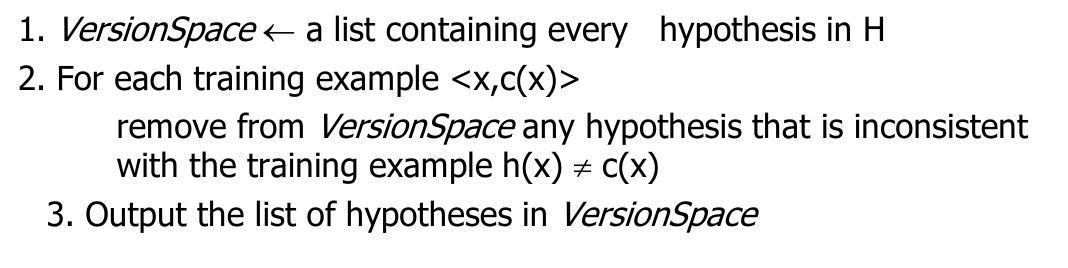
\includegraphics[width=\textwidth]{images/list-then-pseudo}
\end{figure}

\begin{figure}
	\caption{Example of List-Then Algorithm}
	\label{img:list-then}
	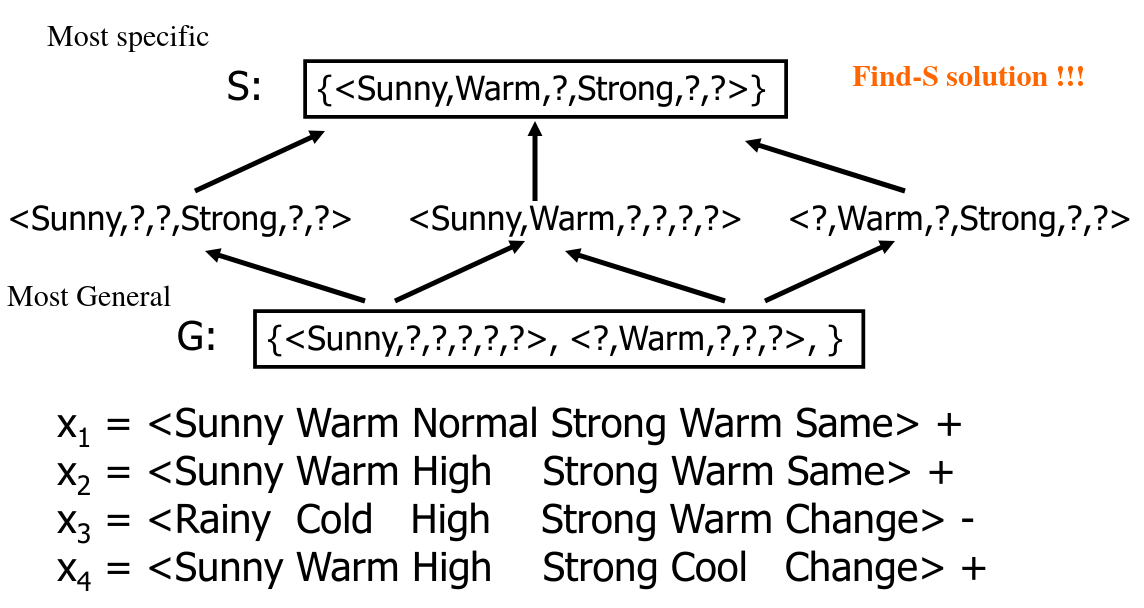
\includegraphics[width=\textwidth]{images/list-then-example}
\end{figure}
To improve list-then we will define two concepts related to version space:
\begin{defi}
The general boundary $G$ of version space is the set of maximally general members (of H consistent with D) and the specific boundary $S$ of version space 
is the set of maximally specific members (of H consistent with D).
\end{defi}

\begin{thm}
	Every member of the version space lies between general and specific boundary
\end{thm}
We can make a complete search of consistent hypotheses using the two boundaries $S$ and $G$ for the $VS$, so we are not restricted to $S$ as for Find-S, and the result can be viewed
in the pseudocode implementation \ref{alg:candidateAlg}.

\begin{figure}
	\caption{Pseudocode of Candidate Eliminate Algorithm}
	\label{alg:candidateAlg}
	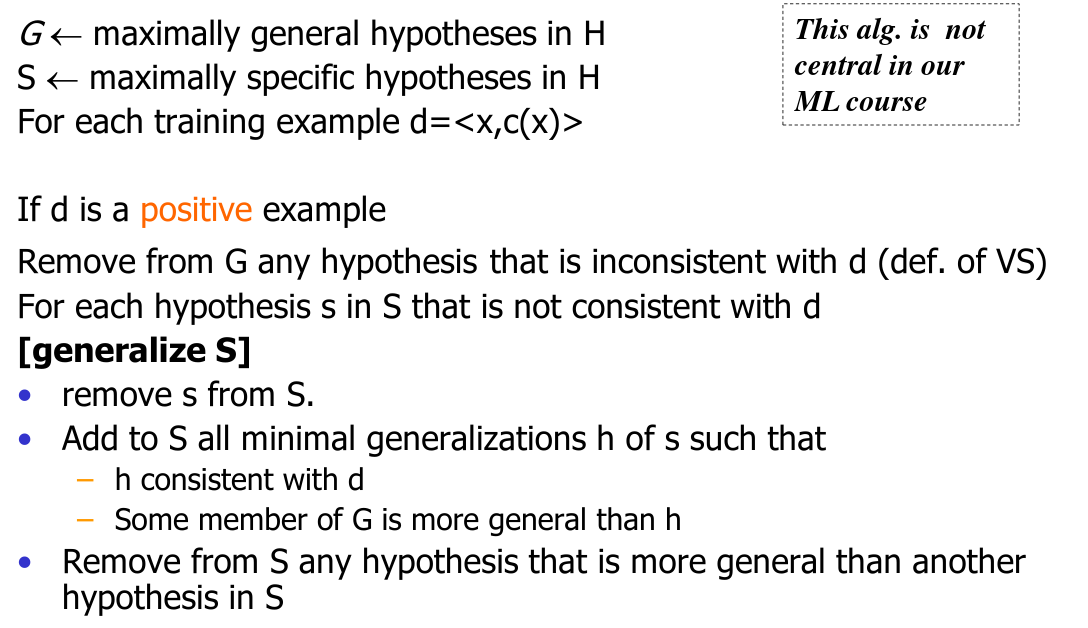
\includegraphics[width=\textwidth]{images/candidateAlg}
	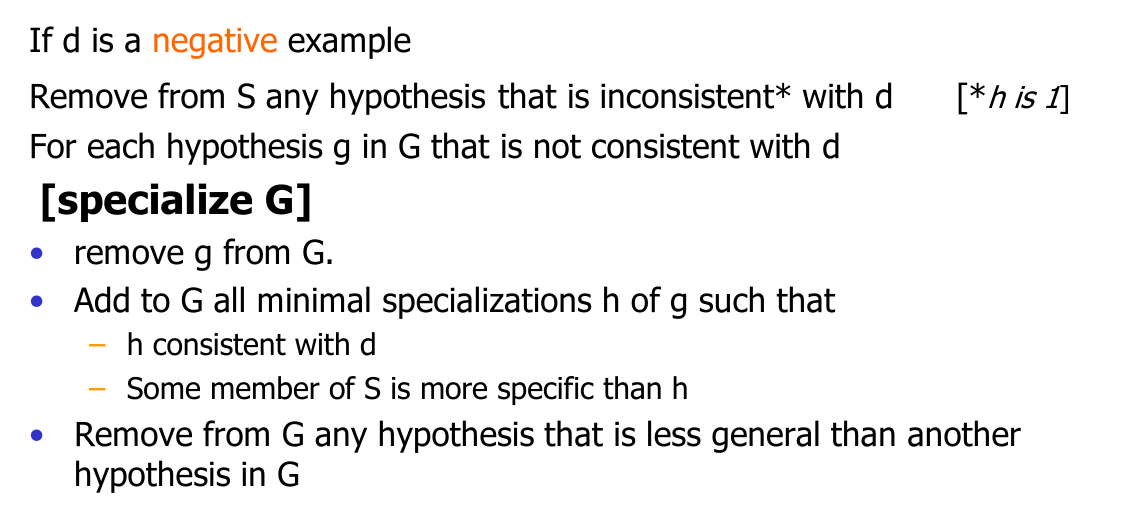
\includegraphics[width=\textwidth]{images/candidatePseudo}
\end{figure}


\section{Inductive Bias}
Our hypothesis space is unable to represent a simple disjunctive target concept so we have some \emph{bias} and we assume that the hypothesis space $H$ contains the target concept, 
in other words that $C$ can be described by a conjunction (AND operator) of literals.

To solve disjunctive target concept we have to choose $H$ that expresses every teachable concept, that means $H$ is the set of all possible subsets of X (power set) and 
assume positive examples $(x1, x2, x3)$ and negative examples $(x4, x5)$ we have that the only examples that are unambiguolsy classified are the training examples themselves (H can represent them).

In other words in order to learn the target concept one would have to present every single instance in X as a training example, so we have that an unbiased Learner is unable to generalize,
infact each unobserved instance will be classified positive by precisely half the hypothesis in VS and negative by the other half (rejection).

A learner that makes no prior assumptions regarding the identity of the target concept has no rational basis for classifying any unseen instances and the (restriction, preference) bias 
not only assumed for efficiency, it is needed for generalization, however does no tell us (quantify) which one is the best solution for generalization.

We define now the \emph{inductive bias} of $L$ is any minimal set of assertions $B$ such that for any target concept $c$ and corresponding training data $D_c$
\[ \forall X_i \in X (B \land D_c \land X_i) \deriv L(X_i, D_c) \]

It is possible to learn rules as a research in discrete hypothesis space and every ML models show an inductive bias, infact learning without an inductive bias
does not allow generalization capabilities and in ML we will look at flexible models with expressive hypothesis spaces (avoiding the language bias) 
focusing on the search bias (which is ruled by the learning algorithm).



